\documentclass{article}

% Language setting
% Replace `english' with e.g. `spanish' to change the document language
\usepackage[french]{babel}

% Set page size and margins
% Replace `letterpaper' with`a4paper' for UK/EU standard size
\usepackage[letterpaper,top=2cm,bottom=2cm,left=3cm,right=3cm,marginparwidth=1.75cm]{geometry}

% Useful packages
\usepackage{amsmath}
\usepackage{graphicx}
\usepackage[colorlinks=true, allcolors=blue]{hyperref}
\usepackage{listings}
\usepackage[section]{placeins}


\title{Outils libres côté client}
\author{Vincent KBIDA - Louis SAGET}

\begin{document}
\maketitle
\tableofcontents
\newpage

\section{TP1 - Efficacité de l'environnement}

\subsection{}

\begin{table}[h]
\centering
\begin{tabular}{l|r}

Description & Raccourci \\\hline
Changer d’onglet sur un terminal & Ctrl + Page up / Ctrl + Page down\\
\hline
Sélectionner un document sur google docs & Espace pour ouvrir le menu des documents\\
 & puis tab pour selectionner le document\\
 \hline
Ouvrir une nouvelle fenêtre de l’élément en cours & Ctrl + shift + N\\
\hline
Définir une zone de capture d’écran & Fn + Maj + Impr.ecran\\
\hline
Commande clear & Ctrl + L\\
\hline
Ajouter un favori sur Firefox & Shift + D\\
\hline
Présentation des onglets ouverts & Super + S\\
\hline
Split vertical tmux & Ctrl+ B puis MAJ + \%\\
\hline
Split horizontale tmux & Ctrl + B puis "\\
\hline
Changement de fenêtre tmux & Ctrl B + Flèches directionnelles\\
\hline
Vérouiller la session & Super + L\\
\hline
Avancer & Tab\\
\hline
Reculer dans un tableau & Shift + Tab\\
\hline
Agrandir / minimiser une fenêtre & Alt + F10


\end{tabular}
\caption{\label{tab:widgets}Raccourcis Linux.}
\end{table}

\subsection{}

Le site \href{https://10fastfingers.com/typing-test/french}{\emph{Fastfingers}} permet d’évaluer la vitesse de frappe.

\begin{figure}[h]
\centering
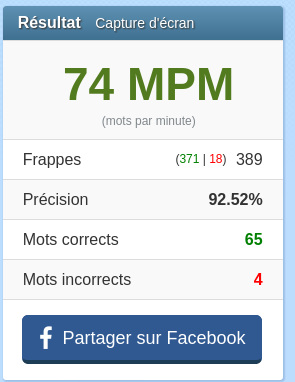
\includegraphics[height=\textwidth]{images/q1-2.jpg}
\caption{\label{fig:frog}Capture d'écran.}
\end{figure}
\FloatBarrier
\subsection{}

\begin{itemize}
    \item Paramétrer GNU Readline pour être en mode Emacs :
    \begin{lstlisting}
    set -o emacs
    \end{lstlisting}
    \item Paramétrer Emacs pour être l’éditeur par défaut :
    \begin{lstlisting}
    update-alternatives --config editor
    \end{lstlisting}
\end{itemize}

\begin{figure}[h]
\centering
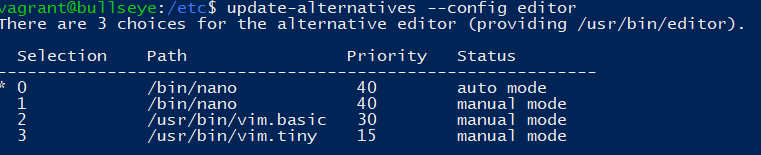
\includegraphics[width=\textwidth]{images/q1-3.jpg}
\caption{\label{fig:frog}Capture d'écran.}
\end{figure}

\subsection{}

\begin{itemize}
    \item L’\emph{history} peut contenir des informations sensibles comme des mots de passe ou d’autres commandes sensibles avec des privilèges élevées. Avoir un \emph{history} court peut signifier que la personne utilise un autre shell (avec un autre \emph{history}) ou que la personne a vidé son \emph{history} (history -c avec des droits appropriés).
    \item Pour éviter de polluer l’\emph{history} avec des commandes simples comme ls, cd ou pwd, on peut utiliser la commande suivante :
    \begin{lstlisting}
    export HISTIGNORE='ls:cd:pwd'
    \end{lstlisting}
    \item Pour remettre ça à zéro tout cela, il suffit de laisser un \emph{history} vide avec la commande suivante :
    \begin{lstlisting}
    export HISTIGNORE=
    \end{lstlisting}
\end{itemize}

\subsection{}

\begin{itemize}
    \item Fonction \emph{mkcd} placée dans le fichier \textasciitilde/.bashrc :
    \begin{lstlisting}
    !#/bin/bash
    mkcd () {
	mkdir $1
	cd $1
    }
    \end{lstlisting}
    \item Fonction \emph{gitemergency} placée dans le fichier \textasciitilde/.bashrc :
    \begin{lstlisting}
    !#/bin/bash
    gitemergency () {
	git add .
	git commit -m "commit d'urgence" $1
	git push
    }
    \end{lstlisting}
\end{itemize}

\subsection{}

\begin{itemize}
    \item Créer un script vide \emph{backup.sh}.
    \item Ajouter le script suivant dans /etc/bash\_completion :
    \begin{lstlisting}
    !#/bin/bash
    _backup() {
    local cur prev opts

    cur="${COMP_WORDS[COMP_CWORD]}"
    prev="${COMP_WORDS[COMP_CWORD-1]}"

    local files=("${cur}"*)

    case $COMP_CWORD in
        1) opts=`getent passwd | cut -d: -f1`;;
        2) opts="now tonight tomorrow";;
        3) opts="${files[@]}";;
        *);;
    esac

    COMPREPLY=()
    COMPREPLY=( $(compgen -W "$opts" -- ${cur}) )
    return 0
    }
    complete -o nospace -F _backup backup
    \end{lstlisting}
\end{itemize}

\subsection{}

Après l’installation de \emph{zsh}, on peut voir dans le fichier .oh\_my\_zsh/themes/[theme\_actuel] de plugin vagrant-prompt son fonctionnement :

\begin{figure}[h]
\centering
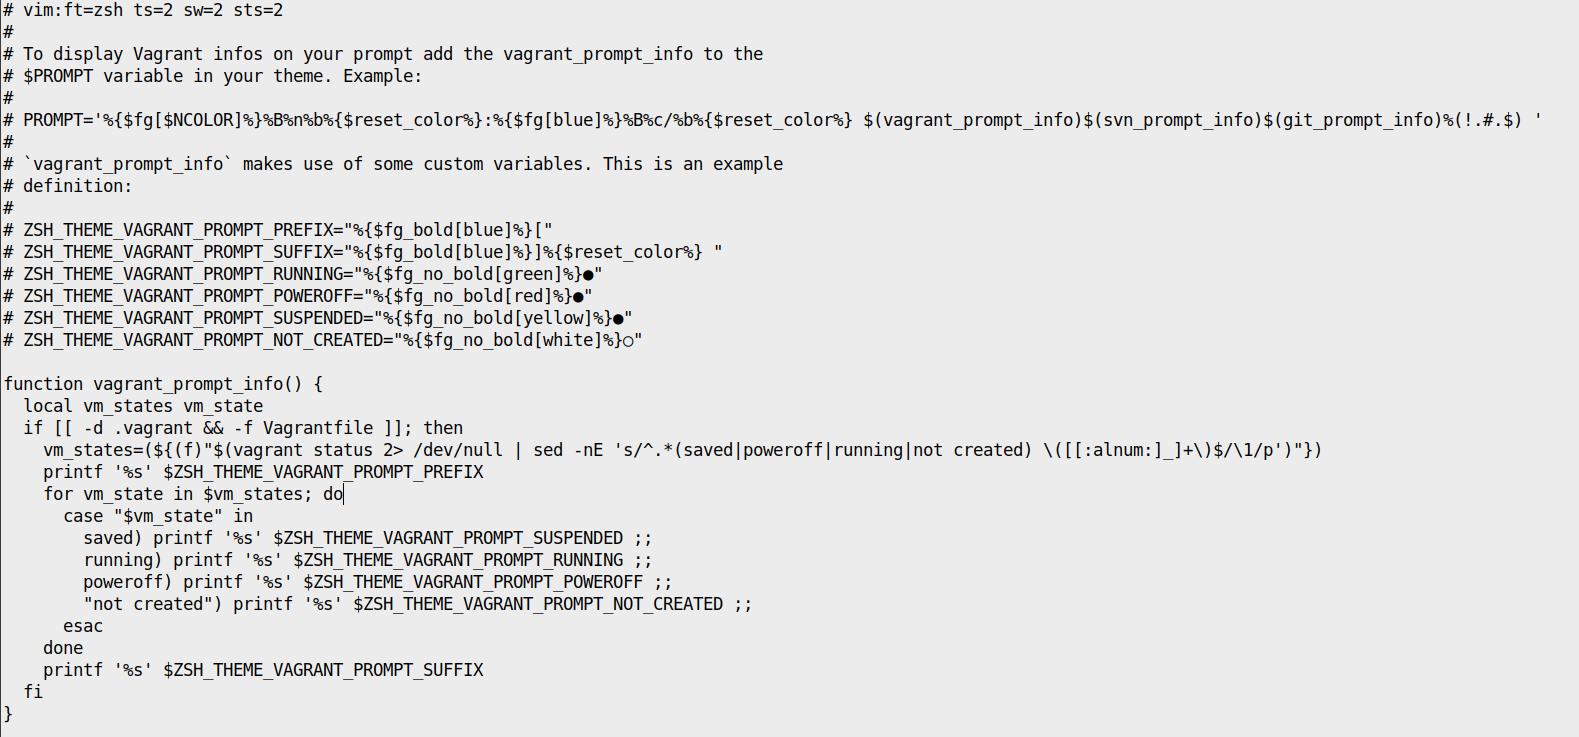
\includegraphics[width=\textwidth]{images/q1-7-1.jpg}
\caption{\label{fig:frog}Capture d'écran.}
\end{figure}

Il suffit ensuite d’ajouter les variables en commentaires au theme actuel dans le fichier \newline
.oh\_my\_zsh/themes/[theme\_actuel] :

\begin{figure}[h]
\centering
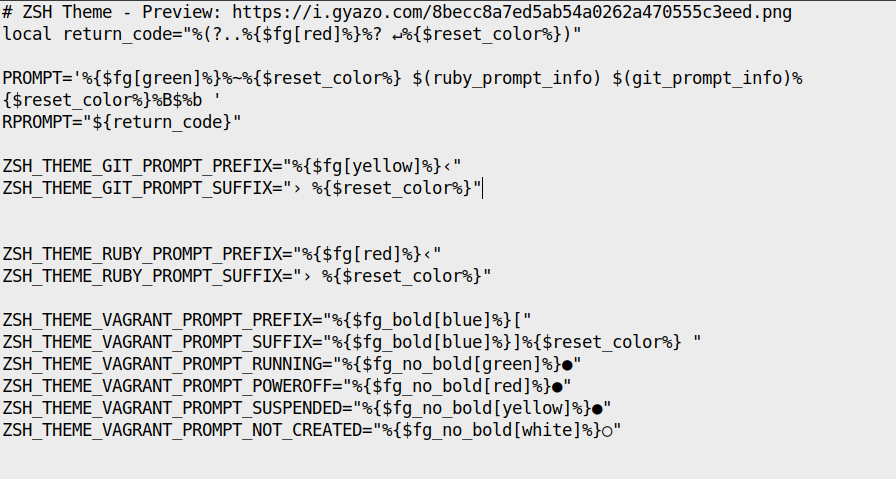
\includegraphics[width=\textwidth]{images/q1-7-2.jpg}
\caption{\label{fig:frog}Capture d'écran.}
\end{figure}

On rajoute le plugin dans le .zshrc et on redémarre zsh :

\begin{figure}[h]
\centering
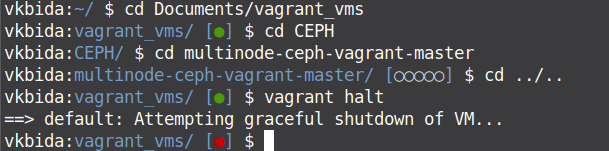
\includegraphics[width=\textwidth]{images/q1-7-3.jpg}
\caption{\label{fig:frog}Capture d'écran.}
\end{figure}

\subsection{}

Script ajouté dans le fichier .zshrc :

\begin{figure}[h]
\centering
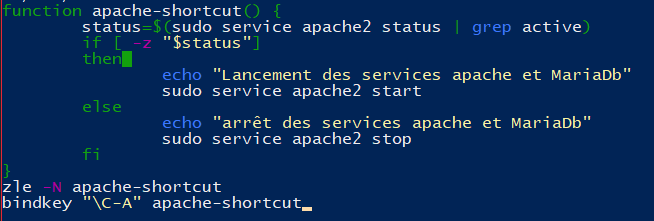
\includegraphics[width=\textwidth]{images/q1-8.jpg}
\caption{\label{fig:frog}Capture d'écran.}
\end{figure}

\subsection{}

\begin{itemize}
    \item Guake :
Peut s’activer et se désactiver avec une touche (F12) -
Transparent -
Coloré.
\item Konsole :
Petit et compact -
Permet de configurer des profils -
Gestion d'onglets.
\item Termit :
Compact -
Gestion des onglets -
Fonction de copier-coller -
Gestion de différentes sessions.
\end{itemize}

\newpage
\section{TP2 - SSH}

\subsection{}

\begin{lstlisting}
ssh alice@10.0.0.3
ssh bob@10.0.0.3
ssh carole@10.0.0.3
\end{lstlisting}

\begin{figure}[h]
\centering
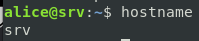
\includegraphics[width=\textwidth]{images/q2-1.jpg}
\caption{\label{fig:frog}Capture d'écran.}
\end{figure}

\FloatBarrier

On constate que l'\emph{history} local est vide car on se connecte pour la première fois sur la session d'un utilisateur d'une nouvelle machine.

\subsection{}

\begin{lstlisting}
cd ~/Documents/Outils_lib/vagrant/
ssh-keygen
ssh-copy-id alice@10.0.0.3
\end{lstlisting}

\begin{figure}[h]
\centering
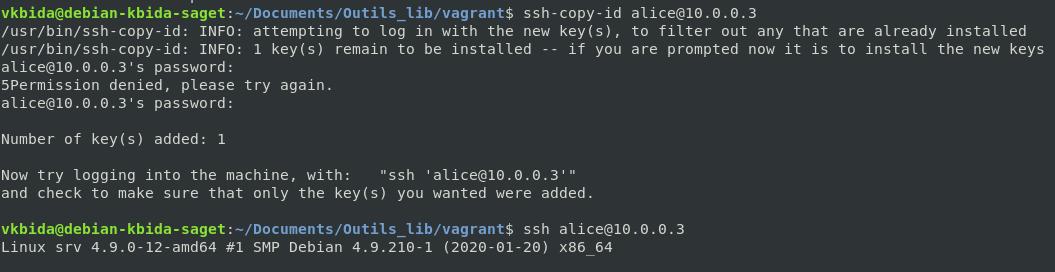
\includegraphics[width=\textwidth]{images/q2-2.jpg}
\caption{\label{fig:frog}Capture d'écran.}
\end{figure}


\begin{lstlisting}
mkdir -p ~/.ssh
cat /vagrant/vag.pub >> ~/.ssh/authorized_keys
\end{lstlisting}

\subsection{}

\begin{itemize}
\item Purger le fichier \textasciitilde/.ssh/known\_hosts :
\begin{lstlisting}
echo "" > ~/.ssh/known_hosts
\end{lstlisting}
\item Ajouter les clés manuellement :
\begin{lstlisting}
cat /vagrant/vag.pub >> ~/.ssh/authorized_keys
\end{lstlisting}
\item Modifier le fichier de configuration SSH :
\begin{lstlisting}
sudo vi ~/.ssh/config
\end{lstlisting}
\item Ajouter :

\begin{lstlisting}
Host bc
	Hostname 10.0.0.3
	User bob
\end{lstlisting}
    \item Connexion via SFTP :
\end{itemize}

\begin{figure}[h]
\centering
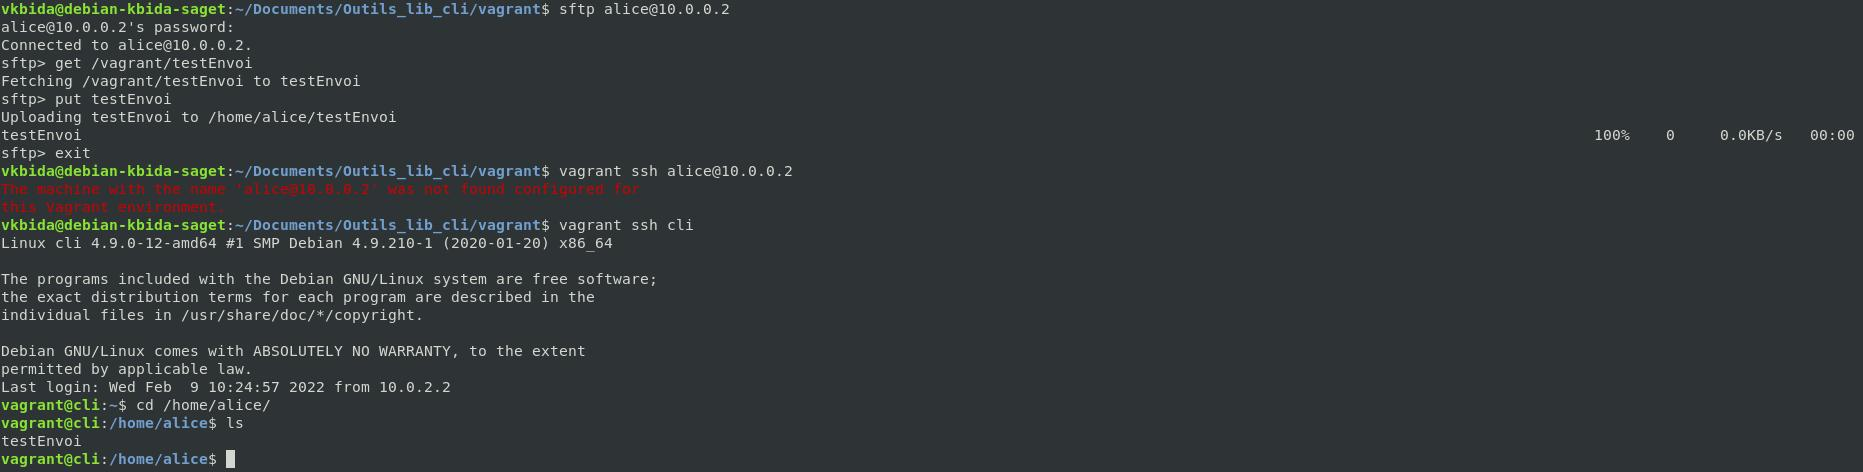
\includegraphics[width=\textwidth]{images/q2-3-1.jpg}
\caption{\label{fig:frog}Capture d'écran.}
\end{figure}

\begin{itemize}
    \item Connexion via SSHFS et vérification :
\end{itemize}

\begin{figure}[h]
\centering
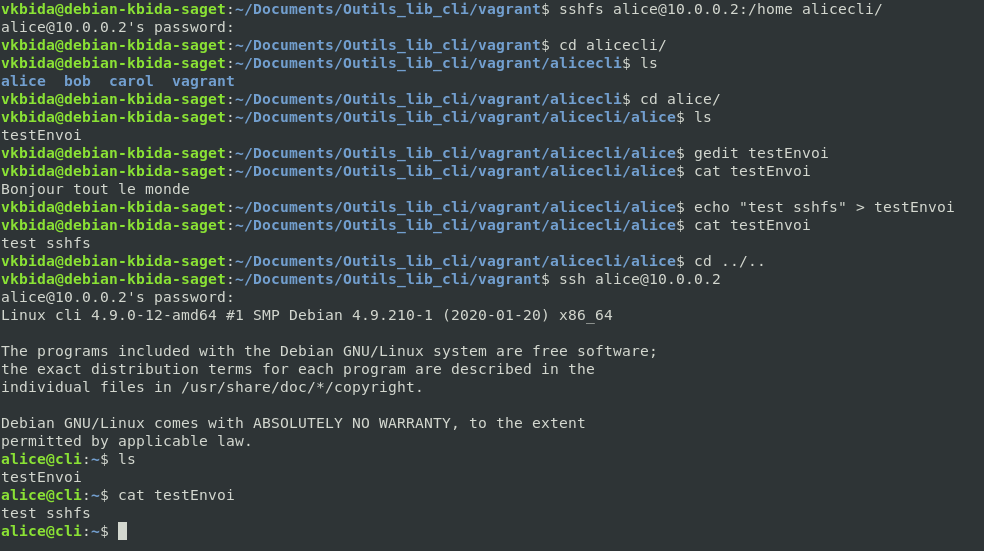
\includegraphics[width=\textwidth]{images/q2-3-2.jpg}
\caption{\label{fig:frog}Capture d'écran.}
\end{figure}

\FloatBarrier

\subsection{}

\begin{itemize}
\item Sur la machine physique :
\begin{lstlisting}
ssh -L 8000:srv.local:80 alice@cli.local
\end{lstlisting}
\item Rester connecté sur \emph{cli.local} avec l’utilisateur alice. Le serveur n’a normalement pas besoin d’utilisateur.
\end{itemize}

\subsection{}

\begin{itemize}
\item Sur la machine physique :
\begin{lstlisting}
ssh -D 9000 srv.local
sudo vi /etc/tsocks.conf
\end{lstlisting}
\item Commenter les lignes suivantes (car \emph{Vagrant} est en local) :
\begin{lstlisting}
#local = 192.168.0.0/255.255.255.0
#local = 10.0.0.0/255.0.0.0
\end{lstlisting}
\item Modifier la ligne suivante :
\begin{lstlisting}
server_port = 9000
\end{lstlisting}
\end{itemize}

\subsection{}

\begin{itemize}
\item Sur la machine cliente :
\begin{lstlisting}
sudo apt install x11-apps
sudo nano /etc/ssh/ssh_config
\end{lstlisting}
\item Modifier la ligne suivante :
\begin{lstlisting}
# ForwardX11 yes
\end{lstlisting}
\item Redémarrer le service :
\begin{lstlisting}
sudo systemctl restart sshd
\end{lstlisting}
\item Sur la machine physique :
\begin{lstlisting}
ssh -X bob@10.0.0.2
xeyes
\end{lstlisting}
\end{itemize}

\subsection{}

\begin{itemize}
\item Sur la machine physique pour le \emph{ProxyJump}, créer le fichier .ssh/config :
\item Ajouter au fichier .ss/config :
\begin{lstlisting}
Host cli
        HostName 10.0.0.2
        User bob

Host srv
        HostName 10.0.0.3
        User alice
        ProxyJump cli
\end{lstlisting}
\item Dans le terminal :
\begin{lstlisting}
ssh srv
\end{lstlisting}
\item Sur la machine physique pour le ProxyCommand, créer le fichier .ssh/config :
\item Ajouter au fichier .ss/config :
\begin{lstlisting}
Host cli
        HostName 10.0.0.2
        User bob

Host srv
        HostName 10.0.0.3
        User alice
        ProxyCommand ssh cli -W %h:%p
\end{lstlisting}
\item Dans le terminal :
\begin{lstlisting}
ssh srv
\end{lstlisting}
\end{itemize}

\newpage
\section{TP3 - Git}

\subsection{}

\begin{figure}[h]
\centering
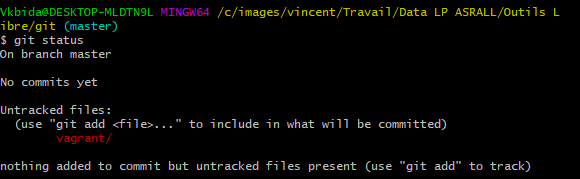
\includegraphics[width=\textwidth]{images/q3-1-1.png}
\caption{\label{fig:frog}Capture d'écran.}
\end{figure}

\begin{figure}[h]
\centering
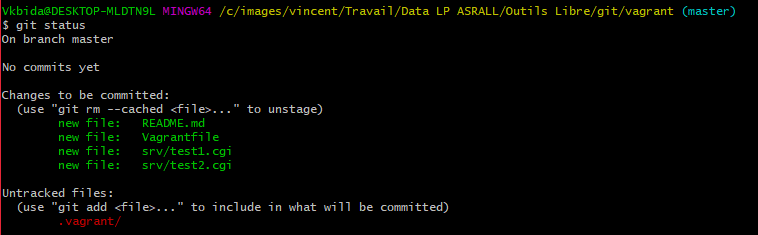
\includegraphics[width=\textwidth]{images/q3-1-2.png}
\caption{\label{fig:frog}Capture d'écran.}
\end{figure}

\begin{figure}[h]
\centering
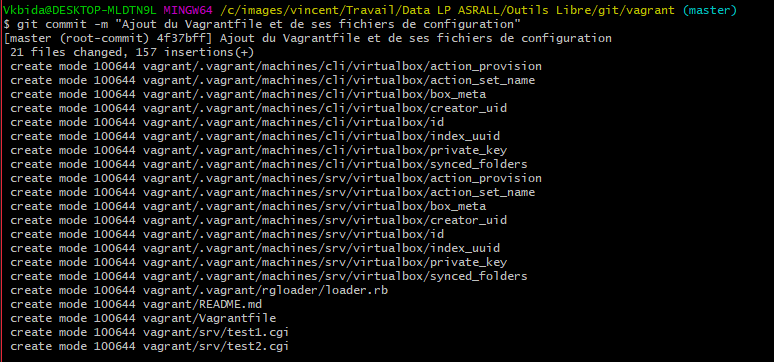
\includegraphics[width=\textwidth]{images/q3-1-3.png}
\caption{\label{fig:frog}Capture d'écran.}
\end{figure}
\FloatBarrier
\subsection{}

\begin{figure}[h]
\centering
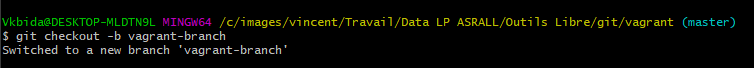
\includegraphics[width=\textwidth]{images/q3-2-1.png}
\caption{\label{fig:frog}Capture d'écran.}
\end{figure}

\begin{figure}[h]
\centering
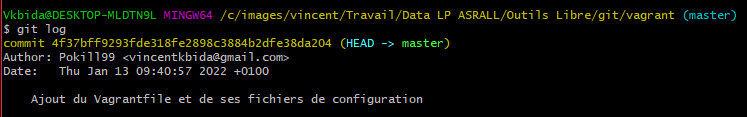
\includegraphics[width=\textwidth]{images/q3-2-2.png}
\caption{\label{fig:frog}Capture d'écran.}
\end{figure}

\begin{figure}[h]
\centering
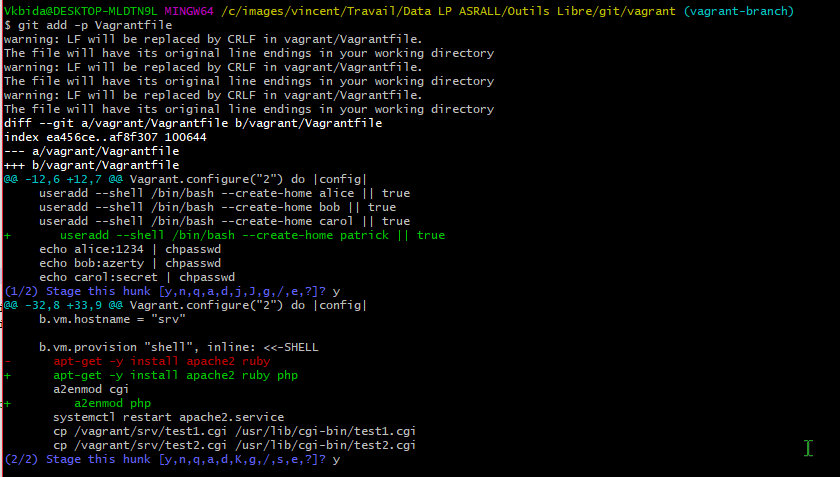
\includegraphics[width=\textwidth]{images/q3-2-3.png}
\caption{\label{fig:frog}Capture d'écran.}
\end{figure}

\begin{figure}[h]
\centering
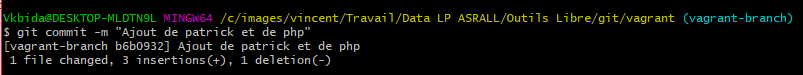
\includegraphics[width=\textwidth]{images/q3-2-4.png}
\caption{\label{fig:frog}Capture d'écran.}
\end{figure}

\begin{figure}[h]
\centering
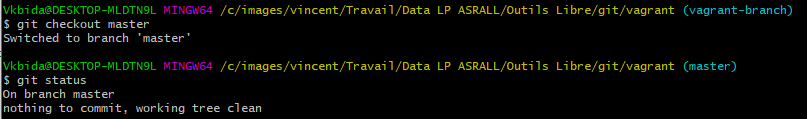
\includegraphics[width=\textwidth]{images/q3-2-5.png}
\caption{\label{fig:frog}Capture d'écran.}
\end{figure}

\begin{figure}[h]
\centering
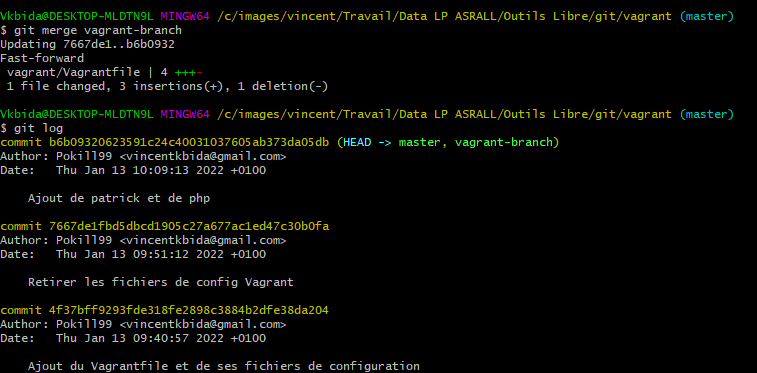
\includegraphics[width=\textwidth]{images/q3-2-6.png}
\caption{\label{fig:frog}Capture d'écran.}
\end{figure}

\begin{figure}[h]
\centering
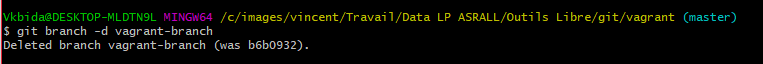
\includegraphics[width=\textwidth]{images/q3-2-7.png}
\caption{\label{fig:frog}Capture d'écran.}
\end{figure}
\FloatBarrier
\subsection{}

\begin{figure}[h]
\centering
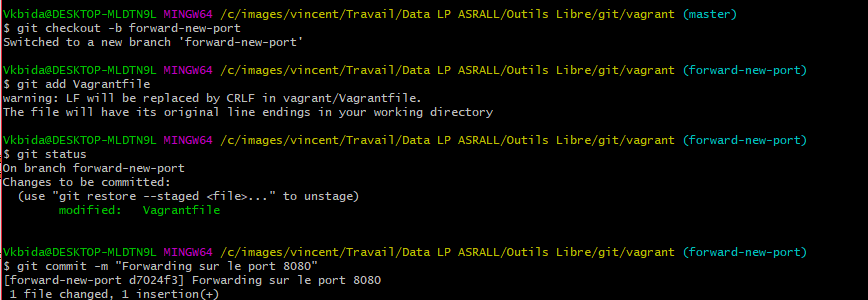
\includegraphics[width=\textwidth]{images/q3-3-1.png}
\caption{\label{fig:frog}Capture d'écran.}
\end{figure}

\begin{figure}[h]
\centering
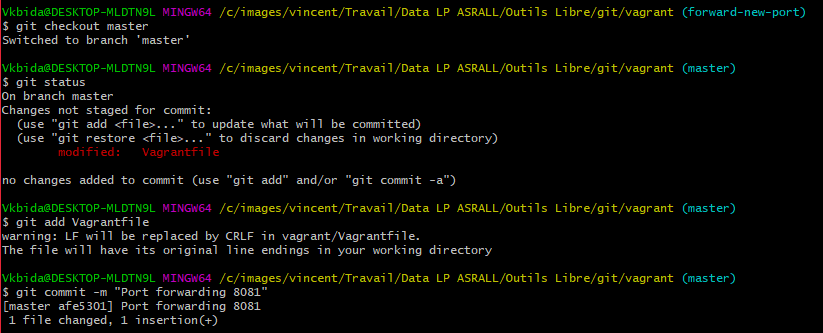
\includegraphics[width=\textwidth]{images/q3-3-2.png}
\caption{\label{fig:frog}Capture d'écran.}
\end{figure}

\begin{figure}[h]
\centering
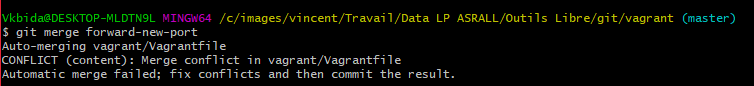
\includegraphics[width=\textwidth]{images/q3-3-3.png}
\caption{\label{fig:frog}Capture d'écran.}
\end{figure}

\begin{figure}[h]
\centering
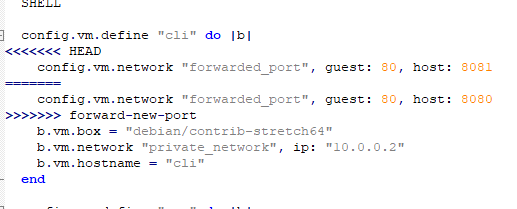
\includegraphics[width=\textwidth]{images/q3-3-4.png}
\caption{\label{fig:frog}Capture d'écran.}
\end{figure}

\bibliographystyle{alpha}
\bibliography{sample}

\end{document}
